\section{Related Work}

\subsection{Infsoft}

Infsoft is a german software company, which specializes in Indoor Tracking, Indoor Positioning and Indoor Navigation. They use custom \emph{infsoft Locator Nodes}\footnote{https://www.infsoft.com/de/technologie/hardware/infsoft-locator-nodes}, which enable to detect the position of devices trough WiFi or Bluetooth, but can also track the location of RFID chips or through Ultra-wideband technology.

This location data is then analyised to track the path of employees, visitors or objects. These analytics are available in real-time over a web interface, which includes a live rendering of a heatmap, showing locations with heavy or low traffic. But also a history of location data can be displayed.
No personal informations get leaked in this system.

\begin{figure}[!hb]
	\centering
	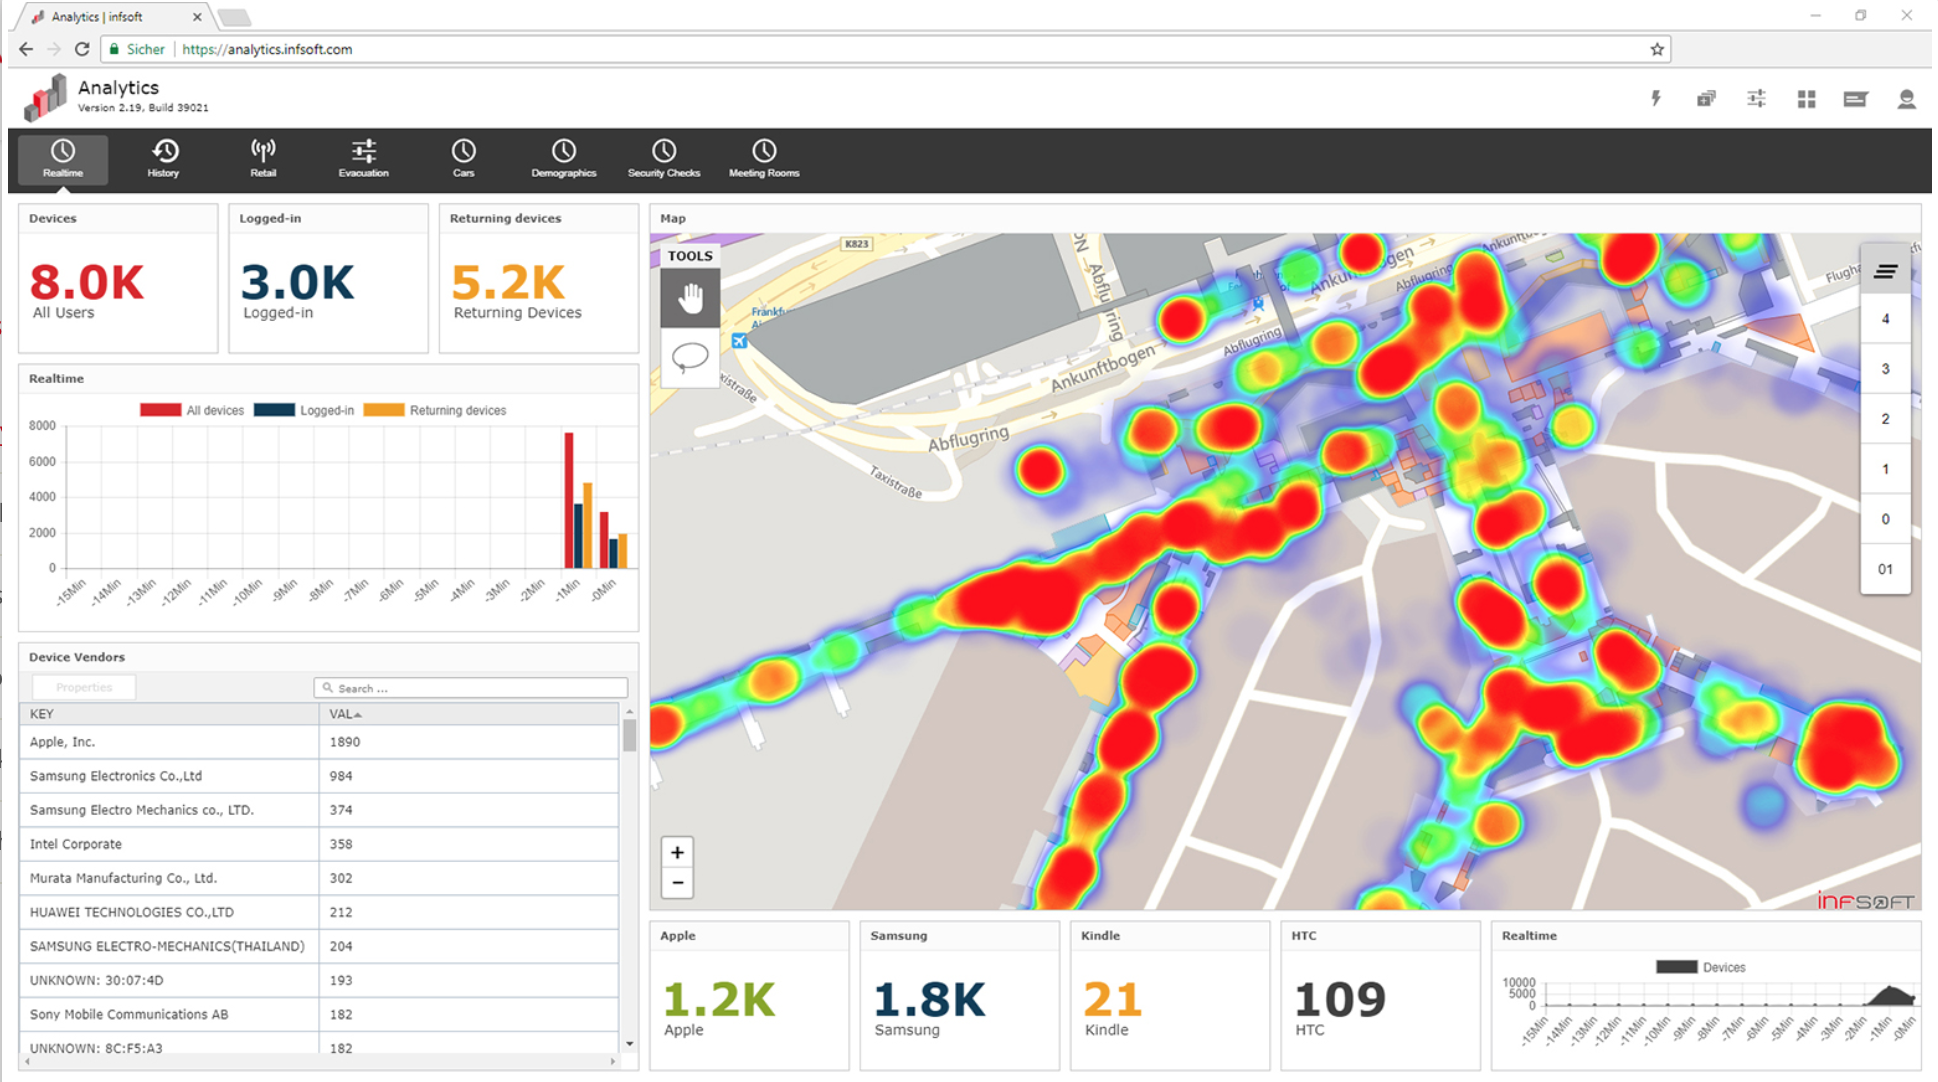
\includegraphics[width=0.9\linewidth]{images/Infsoft}
	\caption{Infsoft Analytics Web Application}
	\label{fig:InfsoftApplication}
\end{figure}

\subsection{Moca}

Moca is a platform for helping companies find out insights about the shopping behaviour of their customers. This contains also analytics about the movement paths of the customers in a shopping mall. Do they go to competitors, how do they get to the store,

To achieve this, they use the existing WiFi network in the building to track the location of the devices, which is accurate. The data then is displayed in real-time floorplan view. They allow real-time playbacks of past days and import of floorplans.

\begin{figure}[!hb]
	\centering
	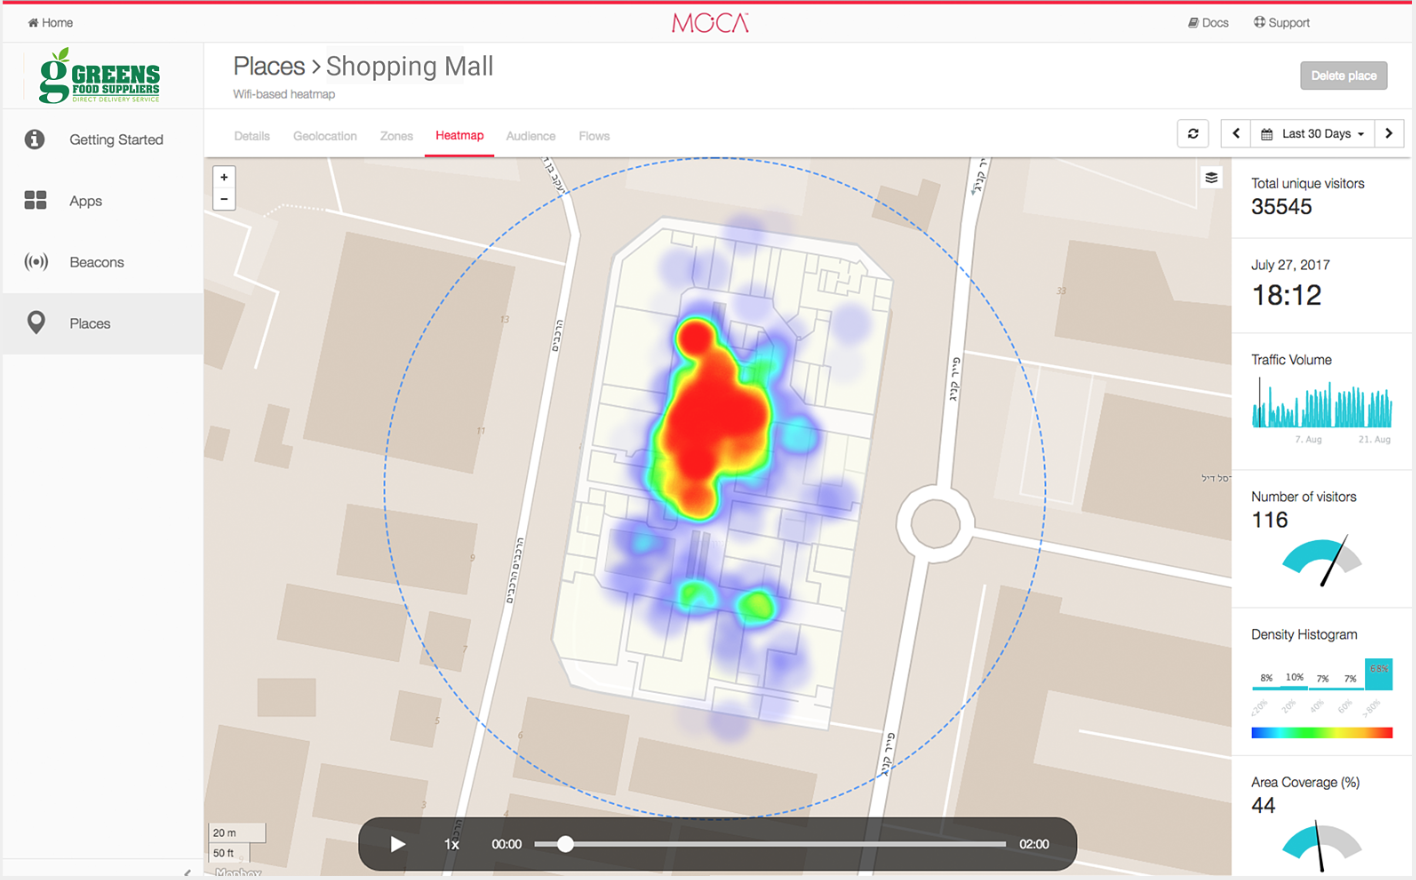
\includegraphics[width=0.9\linewidth]{images/Moca}
	\caption{Moca Web Application}
	\label{fig:InfsoftApplication}
\end{figure}

\subsection{Roommaps}

Einbindung in dritt-anbieter apps.

Auch ueber Wifi + BLE

mehrere stockewekcer und co

navigation

\subsection{Summary}

All these solutions already offer a great set of funtionality. But these are based on the location of devices, which can be determined through a WiFi network or a set of Bluetooth beacons. This makes it unapplicable to our project, because the only data that is available for us are the locations of the gates and the access decisions made at these and not the location of the devices themselves.

Although Roommaps provides their services for third party applications, these services cannot be extended or customized for our use case. 

Additionally, all these services are not open-source products and come with costs regarding hardware and software. Since our project partner requires the use of open-source and free software, the interactive floorplan of our project cannot be based on the related work that was presented and needs to be build from the ground up.

\clearpage